\section{Literatūros apžvalga}\label{sec:literature}

Mokslinėje literatūroje kenkėjiško kodo ir programų obfuskacijai daugiausia dėmesio skiriama \ac{ae} generavimui, dėl paplitusio \acs{ml} modelių naudojimo kenkėjiško kodo ir programų detekcijos srityje \cite{andersonLearningEvadeStatic2018}. Dažniausia atakų platforma -- operacinė sistema \enquote{Windows} ir jos naudojami \acs{pe} formato failai (\href{https://www.virustotal.com/gui/stats}{\textit{VirusTotal}}\footnote{https://www.virustotal.com/gui/stats} duomenimis).

Kenkėjiškų programų analizė gali būti išskiriama į \textbf{statinę analizę} ir \textbf{elgesio (\angl{behavior}) analizę}. Statinės analizės detektoriai yra labiau paplitę ir prieinami, kadangi požymių išskyrimas iš tam tikro iš anksto žinomo formato failų ir jų klasifikavimas yra sąlyginai nesudėtinga užduotis. Tuo tarpu elgesio analizės detektoriai dažniausiai neprieinami eiliniams vartotojams, o diegiami korporacijose \cite{rosenbergGenericBlackBoxEndEnd2018}. Jų veikimas pagrįstas nuolatiniu sistemos stebėjimu ir anomalijų detekcija, tad yra kartu ir sudėtingesnė, ir reikalaujanti daugiau resursų, nei statinė analizė, užduotis.

Mokslinėje literatūroje nagrinėjant specifinį būdą generuoti \acs{ae}, apibrėžiamas \gls{framework}. \Glswhat{framework} sudaro
\begin{itemize}
    \item \Glswhom{surrogateModel} tipas ir architektūra,
    \item \acs{ml} modelio (jei naudojamas) tipas ir architektūra,
    \item \acs{ml} modelio naudojami požymiai (žr. \ref{sec:literature:features}),
    \item \acs{ml} modelio naudojamos perturbacijos (žr. \ref{sec:literature:perturbations}).
\end{itemize}

\subsection{\acs{ae} perkeliamumas}\label{sec:literature:transfer}
Perkeliamumas \acs{di} modeliuose dažniausiai suprantamas kaip žinių perkeliamumas (\angl{knowledge transferability}). Tačiau tiriant \glswhat{adversarial} buvo pastebėtas ir \acs{ae} perkeliamumas (\angl{adversarial sample transferability}). Tai reiškia, jog gebant sukurti \acs{ae}, kuriuos neteisingai klasifikuoja vienas modelis, tikėtina, jog kitas (tos pačios paskirties) modelis taip pat klasifikuos \acs{ae} neteisingai. Be to, nustatyta, jog \acs{ae} perkeliamumo savybė galioja skirtingų architektūrų modeliams \cite{demetrioAdversarialEXEmplesSurvey2021}. Šia savybe remiasi visos \enquote{juodos dėžės} atvejams pritaikytos atakos.
\subsection{Naudojami kenkėjiškų programų požymiai}\label{sec:literature:features}
\Gls{adversarial} taikosi į \acs{ml} modeliais paremtus kenkėjiškų programų detektorius. Šie detektoriai yra klasifikatoriai -- pateiktį (programą) klasifikuoja kaip kenkėjišką (\angl{malicious}) arba nekenkėjišką (\angl{benign}). Kadangi programos nėra fiksuoto dydžio, klasifikatoriai remiasi programų požymiais, kurie gaunami atliekant požymių ištraukimą (\angl{feature extraction}). Laikoma, jog \enquote{juodos dėžės} atvejais sužinoti, kokius tiksliai požymius vertina kenkėjiškų programų detektorius, yra neįmanoma, tad \glsplwhom{framework} apibrėžimuose, priklausomai nuo jų specifikos ir tikslų, neretai pateikiami jų vertinami programų požymiai. Šiame poskyryje išskiriami ir klasifikuojami mokslinėje literatūroje minimi požymiai.

\subsubsection{\acs{pe} formato programų požymiai}\label{sec:literature:features:pe}
\begin{itemize}
    \item \textbf{\acs{dll} vardai (arba \acs{api} vardai \cite{huGeneratingAdversarialMalware2017})} \cite{zhongMalFoxCamouflagedAdversarial2024}. \acs{pe} faile turi būti nurodyti visi naudojami \acs{dll} ir jų \acs{api}. Prieš pradedant mokyti \acs{ml} modelį, atliekama visų turimų programų analizė ir nustatoma visų naudojamų \acs{dll} ar jų \acs{api} aibė $D$. Tarkime $|D| = n$. Tuomet, požymių vektorius programai, naudojančiai $X \subseteq D$ \acs{dll}, bus $n$-matis dvejetainis vektorius, kurio $i$-asis elementas yra $\begin{cases}
        0, \text{ jei } D_i \not \in X, \\
        1, \text{ jei } D_i \in X
    \end{cases}$ čia $D_i$ -- $i$-asis $D$ elementas.
    \item \textbf{\acs{pe} metaduomenys} \cite{andersonLearningEvadeStatic2018}. Tai visi \acs{pe} formato faile esantys metaduomenys, tokie, kaip sekcijų pavadinimai, sekcijų dydžiai, \enquote{ImportTable} ir \enquote{ExportTable} metaduomenys ir kt. Formuojant požymių vektorių skaičiuojama metaduomenų \gls{hashfunction}.
\end{itemize}

\subsubsection{Baitų lygio požymiai (gali būti ištraukiami iš bet kokio formato failų)}\label{sec:literature:features:byte}
\begin{itemize}
    \item \textbf{Prasmingų žodžių (angl. Strings) kiekis} \cite{andersonLearningEvadeStatic2018}. Prasmingus žodžius suprantame kaip turinčius prasmę žmogui \textit{(angl. human readable)}. Tai gali būti URL, failų keliai \textit{(angl. file paths)} ar registro raktų pavadinimai. Kadangi prasmingų žodžių kiekis tėra vienas skaičius, požymių vektorius dažniausiai formuojamas prijungiant ir kitus požymius.
    \item \textbf{Baitų/entropijos histograma} \cite{saxeDeepNeuralNetwork2015}. Specifinis metodas, užkoduojantis dažniausiai pasikartojančias baitų ir entropijos poras $n$ dimensijų vektoriumi.
    \item \textbf{$n$-gramos} \cite{zhuNgramMalGANEvading2022}. Dažniausiai sutinkamos skaitmeniniame natūraliosios kalbos apdorojime (\acs{nlp}). Tai yra $n$ žodžių junginiai, arba, sukompiliuotų programų apdorojimo kontekste, $n$ baitų junginiai. Nustatant požymių vektorių, visos $n$-gramos surikiuojamos pagal pasikartojimą programoje mažėjimo tvarka (\enquote{populiariausios} viršuje). Iš pirmų $m$ reikšmių sudaromas $m$-matis vektorius -- tai ir yra požymių vektorius.
\end{itemize}
\subsection{Perturbacijos}\label{sec:literature:perturbations}

Perturbacijos -- tai pagrindinis obfuskacijos metodas \ac{ae} kūrimui.
Perturbacijų tikslas yra pakeisti kenkėjiškos programos veikimą išsaugant
originalų funkcionalumą. Perturbacijos gali būti sudėtingos ir apimti visą
programą (pvz., visos programos užšifravimas ir pridėjimas prie kitos
programos), semantinės (pvz., tam tikrų mašininio kodo instrukcijų keitimas į
ekvivalentų rezultatą pasiekiančias) arba baitų lygio (pvz., nulinių baitų
pridėjimas programos gale) \cite{huGeneratingAdversarialMalware2017}. Perturbacijų parinkimas įeina į
\glswhom{framework} apibrėžimą. Šiame poskyryje aptariamos mokslinėje
literatūroje minimos perturbacijos.
\subsubsection{Baitų lygio perturbacijos}\label{sec:literature:perturbations:byte}
\begin{itemize}
    \item \textbf{\textit{ARBE} (\textit{Append Random Bytes at the End})} \cite{fangEvadingMalwareEngines2019}. \acs{pe} formato failo gale pridedami atsitiktiniai baitai.
    \item \textbf{\textit{ARI} (\textit{Append Random Import})} \cite{fangEvadingMalwareEngines2019}. \acs{pe} formato failo \textit{ImportAddressTable} lentelėje pridedama atsitiktinai pavadinta biblioteka su atsitiktinai pavadinta funkcija.
    \item \textbf{\textit{ARS} (\textit{Append Randomly named Section})} \cite{fangEvadingMalwareEngines2019}. \acs{pe} formato failo \textit{SectionTable} lentelėje pridedamos atsitiktinės sekcijos (sekcijos ir jų tipai yra apibrėžti \acs{pe} formate).
    \item \textbf{\textit{RS} (\textit{Remove Signature})} \cite{fangEvadingMalwareEngines2019}. Sertifikato pašalinimas iš \acs{pe} formato failo \textit{CertificateTable} lentelės.
    \item \textbf{Naujas įeities taškas} \cite{andersonLearningEvadeStatic2018}. Prasidėjus programai, iškart peršokama nuo naujo įeities taško į originalųjį.
    \item \textbf{\textit{Header Fields}} \cite{demetrioAdversarialEXEmplesSurvey2021}. \acs{pe} formato failo \textit{PE Header} ir \textit{Optional Header} dalių specifinių laukų keitimas (pvz., sekcijos pavadinimo keitimas \cite{andersonLearningEvadeStatic2018}).
    \item \textbf{\textit{Partial DOS}} \cite{demetrioAdversarialEXEmplesSurvey2021}. \acs{pe} formato failo \textit{DOS Header} dalies pirmi 58 baitai po \textit{MZ} skaičiaus yra nenaudojami moderniose operacinėse sistemose, tad juos galima keisti.
    \item \textbf{\textit{Slack Space}} \cite{demetrioAdversarialEXEmplesSurvey2021}. Dėl \acs{pe} formato specifikos, kiekviena nauja sekcija turi prasidėti tam tikro skaičiaus, nurodyto \textit{PE Header} dalyje, kartotiniu nuo pradžios. Kompiliatoriai šį reikalavimą išpildo sekcijų gale pridėdami tiek nulinių baitų, kiek reikia teisingam sulygiavimui pasiekti. Būtent ši nulinių baitų erdvė gali būti keičiama be jokios įtakos originaliai programai.
    \item \textbf{\textit{Padding}} \cite{demetrioAdversarialEXEmplesSurvey2021}. Nulinių baitų pridėjimas failo gale.
    \item \textbf{\textit{Full DOS}} \cite{demetrioAdversarialEXEmplesSurvey2021}. Perturbacijos esmė tokia pat, kaip ir \textit{Partial DOS}, tik naudojami visi \textit{DOS} dalies baitai, išskyrus \textit{MZ} ir \textit{PE Offset} (\textit{Partial DOS} manipuliacijoms naudoja tik dalį tarp \textit{MZ} ir \textit{PE Offset}).
    \item \textbf{\textit{Extend}} \cite{demetrioAdversarialEXEmplesSurvey2021}. Pakeičiama \acs{pe} formato faile \textit{DOS} dalyje esanti \textit{PE Offset} reikšmė į didesnę\footnote{\label{footnote:structure}šios reikšmės padidinimas reiškia visos failo struktūros keitimą (\textit{DOS} dalis yra failo pradžioje). Būtina pakeisti visų sekcijų vietas nuo pradžios (\angl{offset}) jų metaduomenyse.}. Taip padidinama (išplečiama) visa \textit{DOS} dalis. Tolesnis perturbacijos principas yra toks pat, kaip ir \textit{Full DOS}.
    \item \textbf{\textit{Shift}} \cite{demetrioAdversarialEXEmplesSurvey2021}. \acs{pe} formato failuose kiekvienas sekcijos blokas prasideda su sekcijos vieta nuo pradžios (\angl{offset}). Tarkime ši reikšmė yra $S$. Sekcijos kodas pradedamas vykdyti tik nuo adreso $P+S$, kur $P$ -- programos pradžios adresas. Vadinasi, padidinus\footnoteref{footnote:structure} $S$ per $n$, atsiranda $n$ baitų laisvos vietos iki sekcijos pradžios, kurią galima keisti be jokios įtakos programos veikimui.
\end{itemize}
\subsubsection{Semantinės perturbacijos}\label{sec:literature:perturbations:semantic}
\begin{itemize}
    \item \textbf{Nereikalingų \hyperref[feature:dll]{DLL/API vardų} požymių pridėjimas} \cite{huGeneratingAdversarialMalware2017}. \acs{pe} formato faile \textit{ImportTable} lentelėje pridedami originalios programos nenaudojami \acs{dll}/\acs{api} vardai.
    \item \textbf{\textit{Binary Rewriting}} \cite{demetrioAdversarialEXEmplesSurvey2021}. Semantinis instrukcijų perrašymas. Pavyzdžiui, $A+B$ instrukcijos pakeitimas į $A-(-B)$.
\end{itemize}

\subsubsection{Kompleksinės perturbacijos}\label{sec:literature:perturbations:complex}
\begin{itemize}
    \item \textbf{\textit{Obfusmal}} \cite{zhongMalFoxCamouflagedAdversarial2024}. Užšifruojama originalios programos kodo sekcija. Sukuriama ir originalios programos gale pridedama programa \textit{Shell.dll}, kurioje laikomas atšifravimo raktas, originalios programos kodo sekcijos adresas ir dydis. Be to, \textit{Shell.dll} geba atšifruoti originalios programos kodo sekciją ir jai perduoti kontrolę. \textit{Shell.dll} pridedama prie naudojamų \acs{dll}, o programos pradžios taškas nustatomas į \textit{Shell.dll} pradžios tašką. Iliustracija pateikiama \ref{fig:perturbations}-ame pav.
    \item \textbf{\textit{Stealmal}} \cite{zhongMalFoxCamouflagedAdversarial2024}. Visa originali programa užšifruojama ir pridedama prie programos \textit{Shell.exe} galo. \textit{Shell.exe} geba atšifruoti originalią programą ir perduoti jai kontrolę. Iliustracija pateikiama \ref{fig:perturbations}-ame pav.
    \item \textbf{\textit{Hollowmal}} \cite{zhongMalFoxCamouflagedAdversarial2024}. Užšifruojama visa originali programa. Ji pridedama prie kurios nors nekenksmingos programos galo. Prie šio junginio galo pridedama \textit{Hollow.dll} programa, kurios veikiamas panašus į \textit{Shell.exe} iš \textit{Stealmal}. Viso junginio pradžios taškas nustatomas į \textit{Hollowmal.dll} pradžios tašką. Iliustracija pateikiama \ref{fig:perturbations}-ame pav.
\end{itemize}

\begin{figure}[h]
    \begin{small}
        \begin{center}
            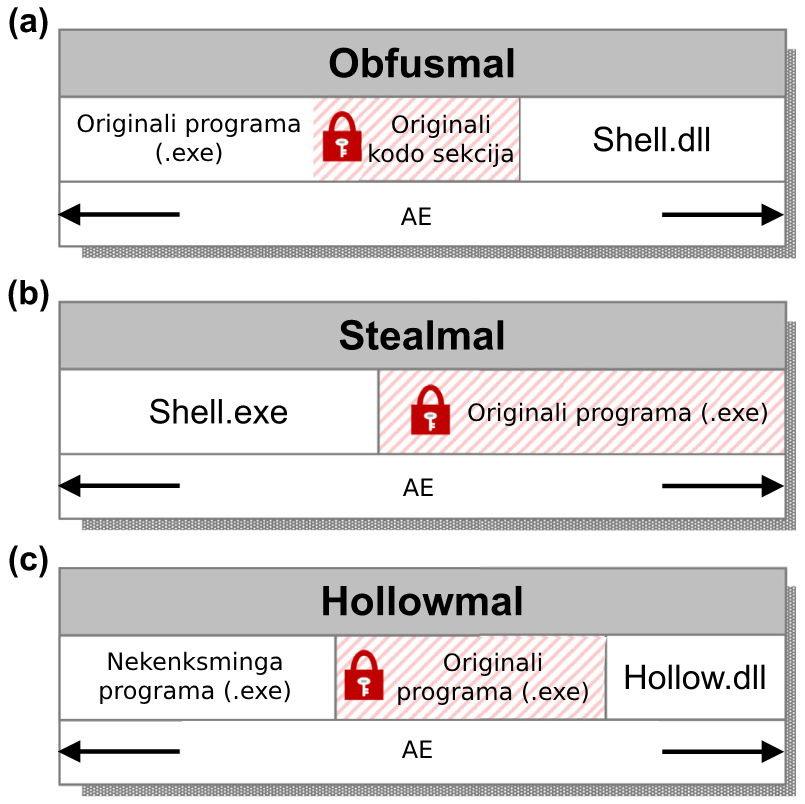
\includegraphics[width=0.95\textwidth]{img/complex-perturbations.png}
        \end{center}
        \caption{Obfusmal (a), Stealmal (b) ir Hollowmal (c) perturbacijų veikimo principų iliustracijos. Adaptuota iš \cite{zhongReinforcementLearningBased2022}}\label{fig:perturbations}
    \end{small}
\end{figure}
\subsection{GAN tipo modelių \glspl{framework}}\label{sec:literature:gan}

\acs{gan} modelių karkasai paremti Generatyviniais Priešiškais Tinklais (\aclp{gan}), kurių veikimo principas yra du neuroniniai tinklai (generatorius ir diskriminatorius), žaidžiantys \gls{zeroSumGame} \cite{chenInfoGANInterpretableRepresentation2016a}. Kenkėjiško kodo obfuskacijos kontekste ir ypač \enquote{juodos dėžės} atvejais, diskriminatorius atlieka \gls{surrogateModel} vaidmenį. Bendras \ac{gan} modelių mokymosi etapas yra tokia seka:
\begin{enumerate}
    \item Generatorius, naudodamas požymių vektorių ir tokios pačios dimensijos
          \enquote{triukšmo} (\angl{noise}) vektorių, sugeneruoja perturbacijas.
    \item Originali kenkėjiška programa modifikuojama pagal perturbacijas (sukuriamas
          \ac{ae}).
    \item Diskriminatorius bando klasifikuoti sugeneruotą \ac{ae} (kenkėjiškas /
          nekenkėjiškas). Diskriminatoriaus klasifikacija lyginama su tikro detektoriaus
          klasifikacija. Jei ji teisinga -- atnaujinami generatoriaus parametrai pagal
          generatoriaus nuostolių funkciją. Kitu atveju, atnaujinami diskriminatoriaus
          parametrai pagal diskriminatoriaus nuostolių funkciją.
    \item Visa seka kartojama nustatytą kiekį kartų.
\end{enumerate} \cite{huGeneratingAdversarialMalware2017,zhuNgramMalGANEvading2022,zhongMalFoxCamouflagedAdversarial2024}.

\begin{describeFramework}{MalGAN}{\cite{huGeneratingAdversarialMalware2017}}
    \introLastPar{
        Tai vienas iš pirmųjų ir populiariausių \acs{gan} tipo modelių \glsplwhom{framework}.
    }
    \purpose{
        Efektyviai išvengti \acs{ae} aptikimo, kai \acs{ml} kenkėjiškų programų detektoriaus implementacija nežinoma (\enquote{juodos dėžės} atvejis)
    }
    \surrogate{
        Daugiasluoksnis tiesioginio sklidimo neuroninis tinklas -- klasifikatorius. Įvestis -- programos požymių vektorius. Išvestis -- klasifikacija į kenksmingą arba nekenksmingą. Šis tinklas taip pat naudojamas kaip diskriminatorius \acs{gan} architektūroje.
    }
    \mainModel{
        Daugiasluoksnis tiesioginio sklidimo neuroninis tinklas. Įvestis -- programos požymių vektorius ir tokios pačios dimensijos \enquote{triukšmo} vektorius. Išvestis -- modifikuotas požymių vektorius. Šis tinklas naudojamas kaip generatorius \acs{gan} architektūroje.
    }
    \features{}{
        \item \textit{MalGan} straipsnyje naudojami tik \acs{api} vardų požymiai, patenkantys į PE formato programų požymių kategoriją (žr. \ref{sec:literature:features:pe}), tačiau autoriai nurodo, jog gali būti naudojami bet kokie požymiai\footnote{\label{footnote:detector-assumptions}autoriai nagrinėja \enquote{juodos dėžės} atvejį su prielaida, jog detektoriaus naudojami požymiai yra žinomi.}.
    }
    \perturbations{}{
        \item Semantinės perturbacijos (\ref{sec:literature:perturbations:semantic}) --
        nereikalingų \acs{api} vardų požymių pridėjimas }
\end{describeFramework}

\begin{describeFramework}{N-gram MalGAN}{\cite{zhuNgramMalGANEvading2022}}
    \introLastPar{
        Šis \glsshort{framework} remiasi \refFramework{MalGAN} karkasu ir siekia jį pagerinti.
    }
    \purpose{
        Supaprastinti, pagreitinti ir pagerinti \glswhat{adversarial}. Pašalinti prielaidas\footnoteref{footnote:detector-assumptions} apie detektorių \enquote{juodos dėžės} atvejais.
    }
    \surrogate{
        Surogatinio modelio veikimas ir architektūra tokia pati, kaip ir \refFramework{MalGAN}
    }
    \mainModel{
        Pagrindinio modelio veikimas ir architektūra labai panašūs į \refFramework{MalGAN}, tačiau norėdami stabilizuoti mokymosi procesą, autoriai siūlo nenaudoti \enquote{triukšmo} vektoriaus. Vietoje to, generatoriaus išvestis ($n$-matis vektorius) modifikuojama nekeičiant pirmų $m$ dimensijų, o kitas $n-m$ pakeičiant nekenksmingų programų požymiais.
    }
    \features{}{
        \item Baitų lygio požymiai (\ref{sec:literature:features:byte}) -- $n$-gramos. }
    \perturbations{Autoriai neatliko eksperimentų su perturbuotomis programomis,
        tačiau pažymi, jog norint gauti sugeneruotus požymių vektorius užtenka pridėti
        reikiamus baitus programos gale. Tai atitinka
        \ref{sec:literature:perturbations:byte} apibrėžtą \vspace{5pt}}{
        \item baitų lygio perturbaciją \textit{ARBE}, tik šiuo atveju pridedami baitai nebūtų
        atsitiktiniai, o norimos $n$-gramos. }
\end{describeFramework}

\begin{describeFramework}{MalFox}{\cite{zhongMalFoxCamouflagedAdversarial2024}}
    \introLastPar{
        \textit{\Name} taip pat remiasi \refFramework{MalGAN}, tačiau siekia kurti \acs{ae} realiomis sąlygomis, dėl to atlieka esminius pakeitimus. 
    }
    \purpose{Generuoti \acs{ae}, kurių neaptiktų komerciniai detektoriai (prieš tai aptarti \glspl{framework} eksperimentams kaip nepriklausomą detektorių naudojo tokius \acs{ml} modelius, kaip \acs{svm}, \acs{knn}, \acs{gbdt} ir kt., bet ne komercinius detektorius). Šio \glswhom{framework} detektorius yra \textit{VirusTotal} (viešai prieinama paslauga, agreguojanti virš 70 komercinių kenkėjiškų programų detektorių).}
    \surrogate{Surogatinis modelis, kaip ir kituose \acs{gan} tipo modelių karkasuose, naudojamas kaip diskriminatorius. Įvestis -- perturbuota programa. Išvestis -- klasifikacija į kenksmingą arba nekenksmingą. Implementacija -- konvoliucinis neuroninis tinklas (\acs{cnn}).}
    \mainModel{Standartinis \acs{gan} generatorius, požymių vektorių sujungiantis su \enquote{triukšmo} vektoriumi. Implementacija -- konvoliucinis neuroninis tinklas (\acs{cnn}).}
    \features{}{
        \item PE formato programų požymiai (\ref{sec:literature:features:pe}) -- \acs{dll}
        vardai. } \perturbations{}{
        \item Visos kompleksinės perturbacijos (\ref{sec:literature:perturbations:complex}) }
\end{describeFramework}
\subsection{Skatinamojo mokymosi tipo modelių karkasai}\label{sec:literature:rl}

Skatinamojo mokymosi (\acs{rl}) modeliai susideda iš agento ir aplinkos. Aplinka susideda iš informatyvių požymių ištraukimo metodo (\textit{angl. feature extraction}) ir kenkėjiškų programų detektoriaus. Agentas -- tai algoritmas ar neuroninis tinklas, kurio tikslas yra surasti optimalią strategiją (\gls{policy}). Šiuo atveju strategija susideda iš perturbacijų (žr. \ref{sec:literature:perturbations}) \citeplace. Bendras \ac{rl} modelių mokymosi etapas yra tokia seka:
\begin{enumerate}
    \item agentas, naudodamas dabartinę aplinkos būseną ir praeito veiksmo atlygį (\textit{angl. reward}), parenka sekantį veiksmą iš galimų veiksmų aibės
    \item atliekamas veiksmas -- perturbuojama programa arba požymių vektorius (priklauso nuo karkaso)
    \item gaunami aplinkos kitimo įverčiai -- nauja būsena ir atlygis, skaičiuojamas pagal detektoriaus klasifikacijos rezultatą
    \item seka kartojama tol, kol agentas nelaiko strategijos optimalia arba nustatytą kiekį kartų
\end{enumerate}
\citeplace{}
\subsection{Genetinių algoritmų tipo modelių \glspl{framework}}\label{sec:literature:genetic}

Genetinai algoritmai (\acs{genetic}) yra viena seniausių mašininio mokymosi
\acs{ml} apraiškų; jų veikimas paremtas evoliucija \cite{castroAIMEDEvolvingMalware2019}. Kenkėjiškų
programų obfuskacijai \acs{ae} generavimas taikant \acs{genetic} yra tokia
seka \cite{yusteOptimizationCodeCaves2022}:
\begin{enumerate}
    \item Sukuriama pradinė populiacija (perturbacijos metodai pradinei populiacijai
          priklauso nuo \glswhom{framework}).
    \item Atliekamas tinkamumo (\angl{fitness}) vertinimas.\label{enum:genetic:fitness}
    \item Atliekama selekcija -- dažniausiai pasirenkami geriausiai įvertinti
          populiacijos \acs{ae}, tačiau galimos ir kitos selekcijos strategijos.
    \item Atliekamas selekcijos atrinktų \acs{ae} kryžminimas (po 2) taip sukuriant naują
          \acs{ae}, turintį po dalį genų iš abiejų kryžmintų \acs{ae}.
    \item Tam tikrai daliai \ac{ae} atliekama dalies genų mutacija.
    \item Vertinama, ar sugeneruoti \acs{ae} atitinka kriterijus (vertina detektorius)
    \item Jei kriterijai nėra tenkinami, seka kartojama nuo \ref{enum:genetic:fitness}-o
          žingsnio.
\end{enumerate}

\begin{describeFramework}{AIMED}{\cite{castroAIMEDEvolvingMalware2019}}
    \purpose{\acs{ae} generavimo greičio padidinimas ir modelių kompleksiškumo sumažinimas, lyginant su \acs{gan} ir \acs{rl} tipo modelių karkasais.}
    \surrogate{Surogatinis modelis nenaudojamas. Naudojami \enquote{juodos dėžės} detektoriai yra \textbf{3 komerciniai} (\textit{Kaspersky, ESET, Sophos}) ir vienas \acs{ml} modelis -- \acs{gbdt}.}
    \mainModel{Klasikinis \acs{genetic} modelis -- veikimas visiškai atitinką bendrą seką. Tinkamumo (\angl{fitness}) vertinamas remiasi \acs{ae} požymių vektoriaus panašumu į originalios programos požymių vektorių (kuo mažiau panašūs, tuo tinkamumo įvertinimas didesnis).}
    \features{}{\item Baitų lygio požymiai (\ref{sec:literature:features:byte}) -- atskiras $n$-gramų
        atvejis, kai $n=1$} \perturbations{}{
        \item Baitų lygio perturbacijos\footnote{autoriai rėmėsi perturbacijomis, aprašytomis
            \cite{andersonLearningEvadeStatic2018}}
        (\ref{sec:literature:perturbations:byte}). }
\end{describeFramework}

\begin{describeFramework}{GAMMA}{\cite{demetrioFunctionalityPreservingBlackBoxOptimization2021}}
    \purpose{Efektyvus (neaptikimo šansų didinmas naudojant perturbacijas, paremtas nekenksmingomis programomis) \glswhose{adversarial} kūrimas.}
    \surrogate{Surogatinis modelis nenaudojamas. \acs{gbdt} ir \textit{MalConv} pasirinkti kaip \enquote{juodos dėžės} detektoriai.}
    \mainModel{Pagrindinė modelio idėja yra požymių ištraukimas iš nekenksmingų programų ir jų pridėjimas, naudojant tam pritaikytas perturbacijas, į kenksmingas programas kiekvienos populiacijos generavimo metu. Tinkamumo (\angl{fitness}) ir kriterijų vertinimas atliekamas naudojant detektorių ir pridėtų požymių dydį baitais (norima pridėti kuo mažiau požymių).}
    \features{}{
        \item \acs{pe} formato programų požymiai (\ref{sec:literature:features:pe}).
        \item Kodas sekcijose (nestandartinis požymis). } \perturbations{}{
        \item Visos baitų lygio perturbacijos (\ref{sec:literature:perturbations:byte}),
        gebančios pridėti baitus.
        \item Autoriai pažymi, jog gali būti naudojama ir \acs{dll} / \acs{api} vardų
        pridėjimo semantinė perturbacija (\ref{sec:literature:perturbations:semantic}).
    }
\end{describeFramework}
\subsection{Nevalidaus PE formato problema}\label{sec:literature:pe_invalid}

Anderson et~al., atlikdami eksperimentus su funkcionalumą išlaikančiomis perturbacijomis \acs{pe} formato failams, pastebėjo, jog ne visais atvejais perturbuotos programos veikia teisingai. Dėl \textit{Windows} operacinės sistemos \acs{pe} formato failų interpretavimo ir paleidimo specifikos, programas įmanoma parašyti tokiu būdu, jog pakeitus kodo ar kitų sekcijų turinį nekeičiant originalių mašininio kodo instrukcijų, programa neveiktų. Techniškai, programų rašymas tokiu būdu pažeidžia patį \acs{pe} formato standartą, tačiau šią praktiką neretai naudoja kenkėjiškų programų autoriai \cite{andersonLearningEvadeStatic2018}.

Norint visiškai išvengti nevalidaus \acs{pe} formato problemos tenka taikyti perturbacijas, nekeičiančias originalių programų, o taikančias kitokius obfuskacijos metodus. Iš \ref{sec:literature:perturbations} poskyryje aptartų perturbacijų, tokias sąlygas atitinka tik 2 kompleksinės perturbacijos (\ref{sec:literature:perturbations:complex}) -- \textit{Stealmal} ir \textit{Hollowmal}.